\documentclass{TDP003mall}
\usepackage{graphicx}


\newcommand{\version}{Version 0.1}
\author{Pontus Haglund, \url{ponha098@student.liu.se}\\
  Niklas Nilsson, \url{nikni292@student.liu.se}}
\title{Kravspecifikation}
\date{2015-11-12}
\rhead{Pontus Haglund\\
Niklas Nilsson}



\begin{document}
\projectpage

\tableofcontents

\newpage

\section{Revisionshistorik}
\begin{table}[!h]
\begin{tabularx}{\linewidth}{|l|X|l|}
\hline
Ver. & Revisionsbeskrivning & Datum \\\hline
0.1 & Dokumentet upprättat & 151112 \\\hline
\end{tabularx}
\end{table}


\section{Beskrivning}
Nedan följer en kort beskrivning av spelet.

\subsection{Kort beskrivning}
Detta projekt kommer skapa en homage till det klassiska spelet missile command. I denna version av missile command kommer spelaren axla ansvaret att försvara en rysk stad från de ondskefulla kapitalisternas anfall med robotar. Spelaren förfogar över en luftvärnsanläggning och har som uppgift att skjuta ner inkommande robotar.

\subsection{Spelarens mål}
Skydda moderlandet från amerikanska robotar som faller från himlen med varierande hastigheter och vinklar. Spelaren skyddar Ryssland från dessa robotar genom att skjuta ner dessa. Spelaren har till sitt förfogande en kanon som denne styr med tangentbordet. Om spelaren misslyckas skjuta sönder inkommande robotar innan dessa träffar staden förstörs en bit av staden. Om hela staden förstörs innan anfallstiden runnit ut så förlorar spelaren. Om staden inte förstörs inom anfallstiden vinner spelaren den nivån och avancerar till en svårare nivå.

\subsection{Kontroller}
\begin{table}[!h]
\begin{tabularx}{\linewidth}{|l|X|}
\hline
Input & Vad händer? \\\hline
Vänster musknapp & Avfyra en robot \\\hline
Muspekaren & Rör siktet som styr var spelarens avfyrade robotar kommer röra sig \\\hline
Esc & Pausar spelet och tar spelaren till en meny \\\hline
\end{tabularx}
\end{table}


\section{Kravspecifikation}
\subsection{Minsta krav}
Nedan följer en tabell med de grundläggande krav som ställs på detta projekt.
\subsubsection{Fienderobotar}
Nedan följer kraven på de fienderobotar som kommer regna från himlen.
\begin{table}[!h]
\begin{tabularx}{\linewidth}{|l|X|}
\hline
Nr & Krav\\\hline
1 & Robotarna ritas ut med sprites på skärmen \\\hline
2 & Robotarna rör sig uppifrån och ner.\\\hline
3 & Vinkeln robotarna rör sig i är slumpmässiga.\\\hline
4 & Hastigheten som robotarna rör sig med är slumpmässig.\\\hline
5 & En svans kommer ritas ut bakom varje robot på skärmen. Denna svans finns kvar till och med roboten förstörs av spelaren eller når marken.\\\hline
6 & När roboten når marken så kommer en explosion ritas ut på skärmen, denna kommer vara animerad.\\\hline
7 & När roboten kolliderar med en projektil från spelarens kanon kommer en explosion att ritas ut, denna kommer vara animerad.\\\hline
8 & Robotarna kan inte kollidera med andra robotar.\\\hline
\end{tabularx}
\end{table}

\newpage

\subsubsection{Spelarens luftvärnsanläggning}
Nedan följer tydliga krav på vad spelarens luftvärnsanläggning skall kunna göra.
\begin{table}[!h]
\begin{tabularx}{\linewidth}{|l|X|}
\hline
Nr & Krav\\\hline
1 & Kanonen kommer ritas ut med en sprite på skärmen.\\\hline
2 & Eldrören kommer visa vilket håll luftvärnet pekar åt.\\\hline
3 & Eldrören kan röras med- och moturs av spelaren med hjälp av muspekaren.\\\hline
4 & Spelaren kan avlossa robotar med hjälp av vänster musknapp.\\\hline
5 & Spelarens eldhastighet är begränsad (antalet robotar per sekund kommer balanseras senare).\\\hline
6 & Robotarna som avlossas av spelaren rör sig med konstanthastighet i riktnigningen som eldrören hade när projektilen avfyrades.\\\hline
7 & När en robot avlossad av spelaren når punkten på skärmen som spelaren siktade på kommer denna att explodera med en animerad explosion.\\\hline
8 & När roboten exploderar tillräckligt nära en fiende robot kommer denna förstöras och en animerad explosion ritas ut.\\\hline
9 & En svans kommer ritas ut bakom spelarens projektiler. Denna försvinner antingen när projektilen lämnar skärmen eller när den förstör en fienderobot.\\\hline
\end{tabularx}
\end{table}

\subsubsection{Staden}
\begin{table}[!h]
\begin{tabularx}{\linewidth}{|l|X|}
\hline
Nr & Krav\\\hline
1 & Staden ritas ut som sprites i form av 6 hus. Staden kommer också ha ryska flaggor.\\\hline
2 & När robotar kolliderar med marken så tar staden skada.\\\hline
3 & Varje gång staden tar skada så kommer detta representeras visuellt av att ett hus i taget blir mer och mer skadat. När huset skadats 2 gånger är detta förstört och ett annat hus kommer förstöras istället.\\\hline
\end{tabularx}
\end{table}

\subsubsection{Diverse}
\begin{table}[!h]
\begin{tabularx}{\linewidth}{|l|X|}
\hline
Nr & Krav\\\hline
1 & Spelet håller ordning på den mängd poäng spelaren skrapar ihop. Dessa visas nere till höger på skärmen och kan också skrivas in spelets high-score.\\\hline
2 & När spelaren är klar med en omgång kan denne spara sin score tillsammans med 3 bokstäver i spelets high-score lista.\\\hline
3 & När spelet startar eller efter en spelomgång är slut skall en splash-screen visas. På denna splash-screen visas high-score listan och texten insert-coin (insert-coin blinkar) or press space-bar to continue. Från denna skräm kommer spelaren till start-menyn.\\\hline
4 & Start-menyn låter spelaren starta spelet med olika svårighetsgrader.\\\hline
5 & Efter en spelomgång är slut men innan high-score skall en besegrad-skärm visas som hånar spelaren.\\\hline
\end{tabularx}
\end{table}

 \newpage
 
\subsection{Extra funktionalitet}
Nedan följer en tabell med extra funktionalitet som i mån av tid kan läggas till i projektet.
\begin{table}[!h]
\begin{tabularx}{\linewidth}{|l|X|}
\hline
Nr & Krav\\\hline
1 & När splash-screen visas spelas sovjethymnen eller internationalen (som en gimmick). \\\hline
2 & Poängen som belönas till spelaren för förstörda robotar baseras på hur tidigt spelaren klarar att skjuta ner dessa i förhållande till när de inträder i spelmiljön. \\\hline
3 & Stadens invånare ritas ut bland husen. Dessa blir mer och mer desperata desto mer skada staden erfar.\\\hline
4 & Specialrobot som gör mer skada, belönar spelaren med fler poäng och bara kommer då och då.\\\hline
5 & Spelaren erhåller erfarenhetspoäng och kan använda dessa för att förbättra olika aspekter av sin kanon.\\\hline
6 & Air force one har flugit fel och råkat flyga in över ditt område. Döda kapitalisternas president och få en stor belöning!\\\hline
7 & Jultomten flyger horisontellt över skärmen och tappar massa julklappar. Skjut sönder klapparna för stora belöningar!\\\hline
8 & Alternativa utseenden för spelet. Här byts alla sprites ut och ger en helt annan känsla till spelet även om funktionaliteten är den samma. Tankar på teman som kan finnas är: 
\newline \newline
Staben command där man är en medlem i staben som skyddar d-nollor från ondskefulla ekonomer. 
\newline \newline
Clown assault, cirkustema där du spelar ett barn som kastar vattenballonger på onda clowner som anfaller.
\newline \newline
Capitalist command, samma som vanliga spelet men här är vi goda kapitalister som försvarar oss mot kommunismens mörka krafter. \\\hline
9 & Alternativa ljud, kan vara bundet till de visuella teman som finns eller helt individuellt\\\hline
\end{tabularx}
\end{table}

\section{Grafik}
Grafiken i detta spel kommer målas upp lager för lager med hjälp av sdl. Vi kommer använda oss av en dubbel buffert där vi bild för bild ritar upp en komplett bild som programmet sedan är redo att visa för spelaren. När det sedan är dags kommer programmet byta till denna färdiga bild och påbörja processen med att rita upp nästa bild. Spelet kommer innehålla utritade bilder som antingen är statiska eller animerade. Med statiska bilder menar vi bilder som inte nödvändigtvis ändras hela tiden. Exempel på detta är till exempel staden som endast förändras till utseendet då fiende robotar träffar marken. Animerade bilder ändras i bestämda intervall. Ett exempel på detta är robotar som har en animerad flamma längst bak.\\\\

Följande sektioner innehåller exempel på den grafik som kommer visas i spelet. All grafik är antingen producerad av oss själva eller används med tillåtelse av upphovsmannen.



\subsection{Statisk grafik}

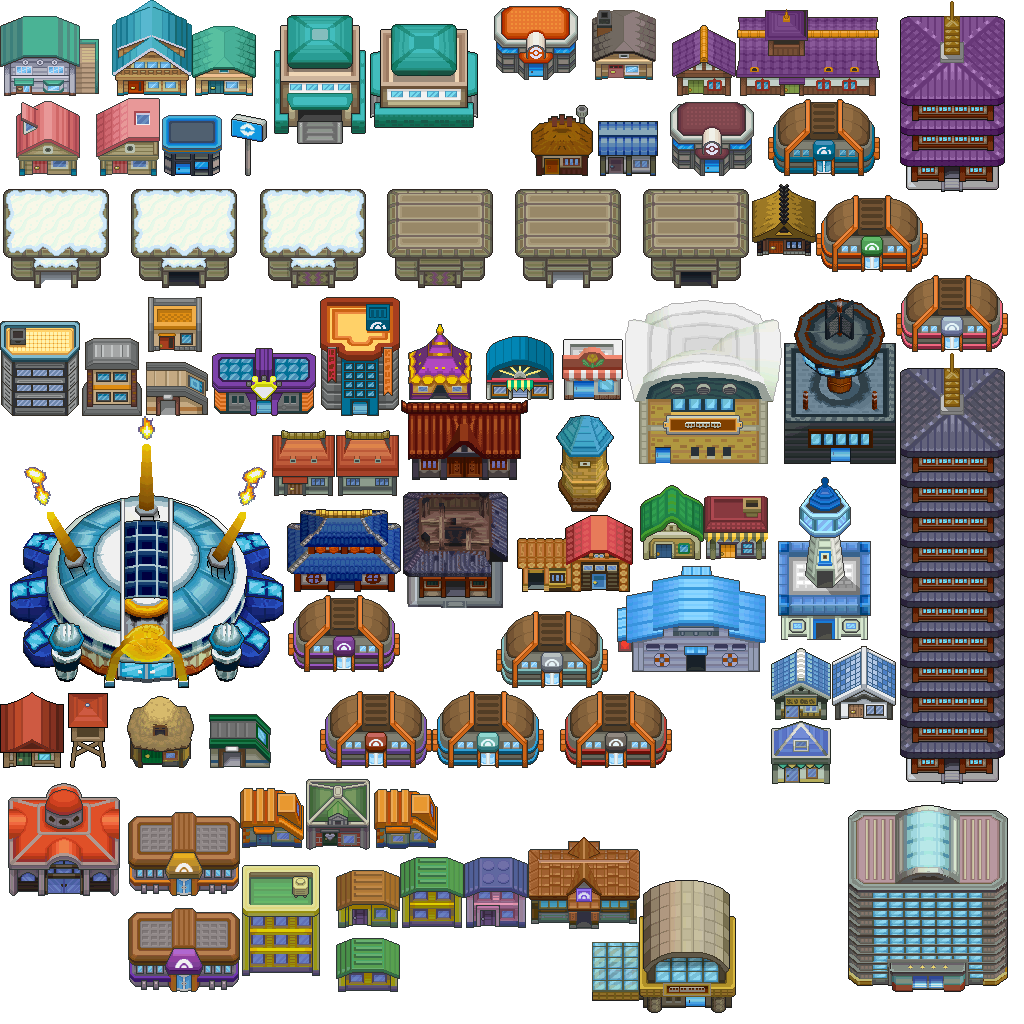
\includegraphics[scale=0.3]{5.png}
\\
Detta är en mockup med bilder som kan användas till husen som skall skyddas

\newpage

\subsection{Animerad grafik}
Nedan visas sådan grafik som animeras.
\\
\includegraphics*[scale=0.4]{4.png}
\\ Exempel på sprites för robotar som faller från himlen och som spelaren skjuter \\\\
\includegraphics*[scale=0.4]{3.png}
\\ Exempel på sprites för robotar som faller från himlen och som spelaren skjuter \\\\
\includegraphics*[scale=0.4]{2.png}
\\ Exempel på animationer för explosioner på marken \\\\
\includegraphics*[scale=0.4]{1.png}
\\ Exempel på animationer på explosioner i luften \\\\



\end{document}
